\documentclass{article}
\addtolength{\oddsidemargin}{-.875in}
\addtolength{\evensidemargin}{-.875in}
\addtolength{\textwidth}{1.0in}
\addtolength{\topmargin}{-0.5in}
\addtolength{\textheight}{1.00in}
\usepackage{wrapfig}
\usepackage{sidecap}
\usepackage{hyperref}
\usepackage[pdftex]{graphicx}
\usepackage[utf8]{inputenc}
\usepackage[spanish]{babel}

\title{Reporte de Actividades - Enero 2019 - Octubre 2021}
\author{Jaime E. Forero Romero\\Profesor Asociado - Departamento de
  F\'isica\\Universidad de los Andes} 
\date{Octubre 7,2021}
\begin{document}

\maketitle
\tableofcontents
\newpage

\section*{Logros principales}
\begin{itemize}
\item Perfil consolidado dentro de Uniandes como docente en programaci\'on, c\'omputo e inteligencia artificial.

\item \'Unico profesor de la Facultad de Ciencias que hace parte del Centro de Investigaci\'on y Formaci\'on en Inteligencia Artificial de Uniandes.

\item Autor de la mayor cantidad de publicaciones en la historia de la astronom\'ia colombiana hasta la fecha. 

\item Perfil profesional de alto reconocimiento y visibilidad dentro de Colombia y Am\'erica Latina.



\end{itemize}

\section{Docencia}

\subsection{Cursos dictados}
\begin{tabular}{p{7.5cm} l c c}\hline
Curso & Semestre & Inscritos \\\hline

F\'isica II & 2019-10 &  84 \\
M\'etodos Computacionales  (viejo p\'ensum) & 2019-10 &  28  \\\hline

M\'etodos Computacionales (viejo p\'ensum) & 2019-20 &   38\\
Herramientas Computacionales (viejo p\'ensum) & 2019-20 &  42 \\\hline

F\'isica II & 2020-10 & 90 \\ 
Introducci\'on a la ciencia de datos & 2020-10 & 15 \\\hline

F\'isica I & 2020-20 & 83 \\
M\'etodos Computacionales I (nuevo p\'ensum) & 2020-20 & 32 \\\hline

F\'isica I & 2021-10 & 75 \\
M\'etodos Computacionales I (nuevo p\'ensum) & 2021-10 & 41 \\\hline

F\'isica I & 2021-20 & 69 \\
M\'etodos Computacionales II (nuevo p\'ensum) & 2021-20 & 22 \\\hline
\end{tabular}

\subsection{Evaluaciones de estudiantes}
\begin{tabular}{l c c }\hline
Semestre & Puntaje & Nivel \\\hline
2019-10 & 4.2/5.0 & promedio-bajo\\\hline
2019-20 & 3.6/5.0 & promedio-bajo\\\hline
2020-10 & sin nota & - \\\hline
2020-20 & 3.8/5.0 & promedio-bajo\\\hline
2021-10 & 3.5/5.0 & promedio-bajo\\\hline
\end{tabular}

\subsection{Desarrollo de nuevos cursos}
\begin{itemize}
\item Construcci\'on de un nueva electiva para pregrado avanzado y posgrado: \emph{Introducci\'on a la ciencia de datos}. 

Programa:

\url{https://github.com/ComputoCienciasUniandes/IntroDataScience/blob/master/programa/programa.pdf}

\item Re-estructuraci\'on de la serie de cursos computacionales para la carrera de F\'isica: \emph{Python Bootcamp} (sin cr\'editos, 16 horas, metodolog\'ia flipped classroom), \emph{M\'etodos computacionales I } (3 cr\'editos, 16 semanas) y \emph{M\'etodos Computacionales II} (2 cr\'editos, 8 semanas).

Programas\\

M\'etodos Computacionales I: \url{https://github.com/ComputoCienciasUniandes/MetComp1_202110/blob/main/programa/programa.pdf}

M\'etodos Computacionales II:
\url{https://github.com/ComputoCienciasUniandes/MetComp2_202120/blob/main/programa/metodos_2.pdf}

Lista de videos\\

Python Bootcamp: 
\url{https://www.youtube.com/playlist?list=PLyCClGzMINigJq71burv1Ci4MVpm2J5se} 


\end{itemize}


\subsection{Direcci\'on de monograf\'ias de pregrado}

\begin{itemize}
\item [5] Jose David Pe\~naranda Rivera, \emph{Detección de supercúmulos de galaxias a partir del flujo de velocidades a gran escala},
  2021-10
 \item [4] Carlos Miguel C\'ordoba Caycedo, \emph{Análisis geométrico de vacíos cósmicos para la acotación de parámetros cosmológicos}. 2020-20. 

\item [3] Diego Andr\'es Torres Guar\'in, \emph{Midiendo la complejidad de la red cósmica}. 2020-20
\item [2] Jairo Andr\'es Saavedra Alonso, \emph{Aprendizaje automatizado para clasificación y estimación de corrimiento al rojo de espectros astrofísicos
}. 2019-
\item [1] Juan Sebasti\'an Barbosa Coy, \emph{Orbits of black holes in galactic triaxial potentials}, 2019-20.  
20.  


\end{itemize}


\newpage
\section{Investigaci\'on}

\subsection{Refereed Papers}

En subrayado sencillo se encuentran estudiantes de pregrado de
Uniandes, en subrayado doble se encuentran estudiantes de posgrado o postdocs bajo mi direcci\'on.

\begin{itemize}

\item[11]{\it Cosmic Velocity Field Reconstruction Using Artificial Intelligence}. 

Wu, Ziyong ; Zhang, Zhenyu ; Pan, Shuyang ; Miao, Haitao ; Luo, Xiaolin ; Wang, Xin ; Sabiu, Cristiano G; \textbf{Forero-Romero, Jaime}; Wang, Yang; Li, Xiao-Dong.

The Astrophysical Journal, Volume 913, Issue 1, id.2, 10 pp, May 2021

\url{https://iopscience.iop.org/article/10.3847/1538-4357/abf3bb}

\item[10]{\it Superclusters from velocity divergence fields}.

\underline{Pe\~naranda-Rivera, J. D.} ; Paipa-León, D. L. ; Hernández-Charpak, S. D. ; \textbf{Forero-Romero, J. E.}

Monthly Notices of the Royal Astronomical Society: Letters, Volume 500, Issue 1, pp.L32-L36, January 2021

\url{https://academic.oup.com/mnrasl/article-abstract/500/1/L32/5948101}

\item[9]{\it Classifying image sequences of astronomical transients with deep neural networks}.

Gómez, Catalina; Neira, Mauricio ; Hernández Hoyos, Marcela ; Arbeláez, Pablo ; \textbf{Forero-Romero, Jaime E.}

Monthly Notices of the Royal Astronomical Society, Volume 499, Issue 3, pp.3130-3138, December 2020

\url{https://academic.oup.com/mnras/article-abstract/499/3/3130/5917433}.  

\item[8]{\it The cosmic web through the lens of graph entropy}.

\underline{García-Alvarado, M. V.} ; Li, X. -D. ; \textbf{Forero-Romero, J. E.} 
Monthly Notices of the Royal Astronomical Society: Letters, Volume 498, Issue 1, pp.L145-L149, November 2020

\url{https://academic.oup.com/mnrasl/article-abstract/498/1/L145/5894926}. 

\item[7]{\it Cosmological parameter estimation from large-scale structure deep learning}. 

Pan, ShuYang ; Liu, MiaoXin ; \textbf{Forero-Romero, Jaime} ; Sabiu, Cristiano G. ; Li, ZhiGang ; Miao, HaiTao ; Li, Xiao-Dong

Science China Physics, Mechanics \& Astronomy, Volume 63, Issue 11, article id.110412, September 2020

\url{https://link.springer.com/article/10.1007%2Fs11433-020-1586-3}. 


\item[6]{\it MANTRA: A Machine-learning Reference Light-curve Data Set for Astronomical Transient Event Recognition}, 

Neira, Mauricio; Gómez, Catalina ; \underline{\underline{Suárez-Pérez, John F.}} ; Gómez, Diego A. ; Reyes, Juan Pablo ; Hoyos, Marcela Hernández ; Arbeláez, Pablo ; \textbf{Forero-Romero, Jaime E.}

The Astrophysical Journal Supplement Series, Volume 250, Issue 1, id.11, 13 pp., September 2020

\url{https://iopscience.iop.org/article/10.3847/1538-4365/aba267}.

\item[5]{\it Using the Mark Weighted Correlation Functions to Improve the Constraints on Cosmological Parameters}.  

Yang, Yizhao ; Miao, Haitao ; Ma, Qinglin ; Liu, Miaoxin ; Sabiu, Cristiano G. search by orcid ; \textbf{Forero-Romero, Jaime}; Huang, Yuanzhu ; Lai, Limin ; Qian, Qiyue ; Zheng, Yi ; Li, Xiao-Dong

The Astrophysical Journal, Volume 900, Issue 1, id.6, September 2020

\url{https://iopscience.iop.org/article/10.3847/1538-4357/aba35b}.

\item[4]{\it Dark matter halo shapes in the Auriga simulations}.

 \underline{\underline{Prada, Jesus}} ; \textbf{Forero-Romero, Jaime E.} ; Grand, Robert J. J.; Pakmor, Rüdiger; Springel, Volker

Monthly Notices of the Royal Astronomical Society, Volume 490, Issue 4, p.4877-4888, December 2019

\url{https://academic.oup.com/mnras/article-abstract/490/4/4877/5586599}.

\item[3]{\it $\beta$-Skeleton analysis of the cosmic web}.

Fang, Feng ; \textbf{Forero-Romero, Jaime} ; Rossi, Graziano ; Li, Xiao-Dong ; Feng, Long-Long

Monthly Notices of the Royal Astronomical Society, Volume 485, Issue 4, p.5276-5284, June 2019

\url{https://academic.oup.com/mnras/article-abstract/485/4/5276/5420836}.

\item[2] {\it Correcting for fibre assignment incompleteness in the DESI Bright Galaxy Survey}. 

Smith, Alex ; He, Jian-hua; Cole, Shaun; Stothert, Lee ; Norberg, Peder ; Baugh, Carlton ; Bianchi, Davide ; Wilson, Michael J. ; Brooks, David ; \textbf{Forero-Romero, Jaime E.} ; Moustakas, John; Percival, Will J. ; Tarle, Gregory ; Wechsler, Risa H.

Monthly Notices of the Royal Astronomical Society, Volume 484, Issue 1, p.1285-1300, March 2019

\url{https://academic.oup.com/mnras/article-abstract/484/1/1285/5281295}.


\item[1] {\it Lyman $\alpha$ photons through rotating outflows}. 

\underline{Remolina-Gutiérrez, Maria Camila} ; \textbf{Forero-Romero, Jaime E.}

Monthly Notices of the Royal Astronomical Society, Volume 482, Issue 4, p.4553-4561, February 2019

\url{https://academic.oup.com/mnras/article-abstract/482/4/4553/5173108}.

\end{itemize}


\newpage
\subsection{Bibliometr\'ia}
\begin{figure}[!h]
\begin{center}
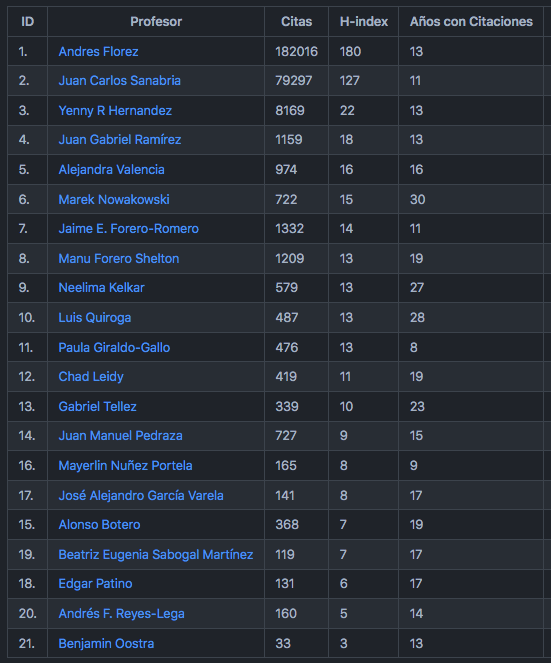
\includegraphics[scale=0.55]{scholar_fisica.png}
\caption{
El impacto de mi producci\'on investigativa se clasifica en el {\bf segundo cuartil de los profesores de planta del departamento de F\'isica} en
  un ranking decreciente por H-index. 
  En esta clasificaci\'on se toman en cuenta los resultados de
  perfiles p\'ublicos de Google Scholar
  para los \'ultimos cinco a\~nos de citaciones solamente, esto con el
  inter\'es de descontar el efecto de investigadores con m\'as a\~nos de
  actividad y comparar con mejor paridad la productividad
 y el impacto  reciente. Esta tabla se encuentra en: \url{https://github.com/forero/gsc/blob/master/info/fisica_uniandes.md}\label{table:fisica}}
\end{center}
\end{figure}

\newpage

\begin{figure}[!h]
\begin{center}
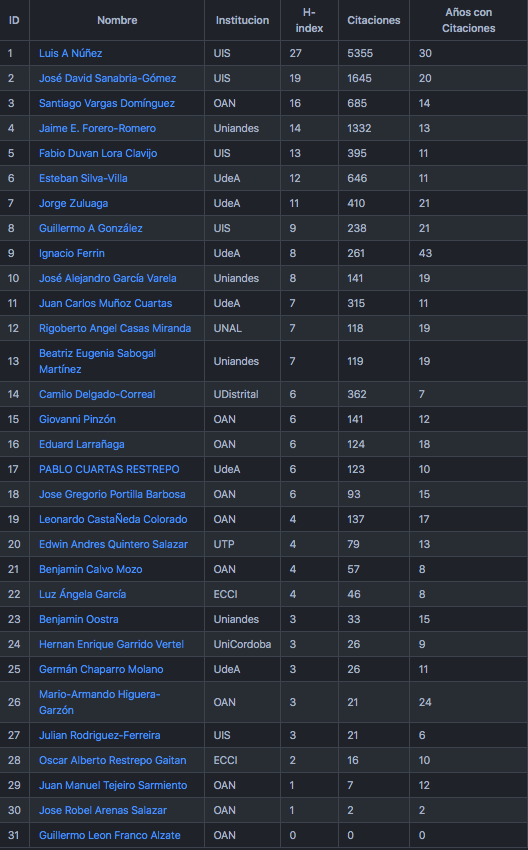
\includegraphics[scale=0.55]{scholar_astronomia.png}
\caption{
El impacto de mi producci\'on investigativa se clasifica en el {\bf cuartil
  superior de todos los investigadores colombianos en el \'area de
  astronom\'ia y astrof\'isica} en 
  un ranking decreciente por H-index. 
  En esta clasificaci\'on se toman en cuenta los resultados de
  perfiles p\'ublicos de Google Scholar
  para los \'ultimos cinco a\~nos de citaciones solamente, esto con el
  inter\'es de descontar el efecto de investigadores con m\'as a\~nos de
  actividad y comparar con mejor paridad la productividad
  reciente. 
Esta tabla se encuentra en: 
\url{https://github.com/ColombianAstronomy/ProductividadAstronomica/blob/master/google_scholar.md}
\label{table:astro}}
\end{center}
\end{figure}


\begin{figure}[!h]
\begin{center}
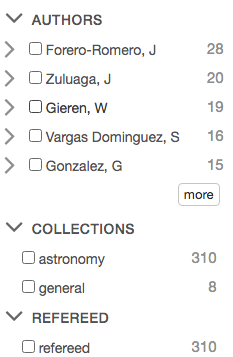
\includegraphics[scale=0.55]{colombia_ADS.png}
\caption{En toda la historia de la astronom\'ia colombiana se han publicado 310 papers. El top 5 de autores se presenta en la imagen (obtenida desde \url{http://adsabs.harvard.edu/}) junto al n\'umero total de publicaciones que se han hecho desde instituciones colombianas por los autores listados.
Desde que soy profesor de Uniandes en el 2012 he logrado publicar 28 papers, un n\'umero mayor que cualquier otro investigador en la historia del pa\'is. J. Zuluaga es profesor en la UdeA desde el 2008. W. Gieren fue profesor en Uniandes en la d\'ecada de los 80. S. Vargas-Dominguez (egresado Uniandes, antiguo postdoc del grupo de astronom\'ia de Uniandes) es profesor en el Observatorio Astron\'omico Nacional desde el 2015. G. Gonz\'alez es profesor en la UIS desde el 2006.
Esta tabla se puede acceder desde : 
\url{https://github.com/ColombianAstronomy/ProductividadAstronomica/blob/master/ads_institutions.md}
\label{table:astro}}
\end{center}
\end{figure}

\newpage

\subsection{Asesor\'ia posgrado}

Doctorado:
\begin{itemize}

\item [1] John Fredy Su\'arez. Examen de conocimientos aprobado en 2019-10. Co-autor en un paper ya publicado. Primer autor en un paper aceptado en Septiembre 2021. Fecha esperada de graduaci\'on: Diciembre 2021.
\item [3] Yeimy Camargo. Estudiante de doctorado en la Universidad Nacional de Colombia
  Sede Bogot\'a. Fecha esperada de graduaci\'on: Diciembre 2021.
\end{itemize}

Maestr\'ia:
\begin{itemize}
\item [3] Felipe G\'omez, \emph{Beta-Voids: Un Identificador de Vacíos Cosmológicos en la Estructura de Gran Escala para Catálogos de Galaxias Basado en el Grafo Beta-Skeleton
}, Diciembre 2019.
\end{itemize}


\subsection{Asesor\'ia de postdocs}

\begin{itemize}
\item David Sierra-Porta. 2020-2021. Como resultado principal tenemos una publicaci\'on env\'iada en Septiembre 2020 a una revista de primer cuartil.

\end{itemize}

\newpage
\subsection{Financiaci\'on}

Durante el 2019 terminamos el siguiente proyecto de COLCIENCIAS\\

\begin{tabular}{l l l p{2.4cm} p{4.0cm} c}\hline
N$^{o}$ & Fecha & Duraci\'on & Instituci\'on & Proyecto & Monto \\\hline

1 & 1.10.2016 & 36 meses & COLCIENCIAS & Simulaciones y Observaciones del Universo a Gran Escala & 200 Millones COP\\\hline
\end{tabular}

\vspace{0.5cm}

Durante el 2019 terminamos el siguiente proyecto interdisciplinario de vicerrector\'ia de investigaciones de Uniandes\\

\begin{tabular}{l l l p{2.4cm} p{4.0cm} c}\hline
N$^{o}$ & Fecha & Duraci\'on & Instituci\'on & Proyecto & Monto \\\hline
2 & 1.10.2017 & 24 meses & Uniandes & 
Spatio-Temporal Transient Object Localization in Astronomical Image
Sequences Using Machine Learning & 84 Millones COP \\
\end{tabular}


\vspace{0.5cm}

Durante el 2019 continuamos con la ejecuci\'on del siguiente proyecto de la Uni\'on Europea (la ejecuci\'on se paus\'o durante el 2020 y 2021, y cerrar\'a  en el 2022)\\

\begin{tabular}{l l l p{2.4cm} p{4.0cm} c}\hline
N$^{o}$ & Fecha & Duraci\'on & Instituci\'on & Proyecto & Monto \\\hline
2 & 1.03.2017 & 48 meses & Uni\'on Europea & Latin-American Galaxy Formation Network \url{https://www.lacegal.com/} & 1.4 Millones EURO \\\hline
\end{tabular}

\subsection{Visitas de investigaci\'on}
\begin{tabular}{p{1.7cm} p{1.3cm} p{2.0cm} p{1.5cm} p{7.0cm}}\hline
Date & Duration & Country & City & Institute\\\hline
Junio 2019 & 4 semanas & UK & Durham & Institute for Computational Cosmology\\
Julio 2019 & 4 semanas & Alemania & Munich & Max Planck Institute for Astrophysics\\\hline
\end{tabular}

\subsection{Colaboraciones Internacionales de Alto Impacto}

\begin{itemize}

\item Dark Energy Spectroscopic Instrument (DESI).

Proyecto de \'ultima generaci\'on de cosmolog\'ia observacional.
El proyecto tiene un costo de hardware de 50 millones de d\'olares. Se esperaba que empezara a tomar datos en el 2020, pero debido a la pandemia el experimento empez\'o en el 2021 y tomar\'a datos hasta el 2026.
El proyecto es liderado por Lawrence Berkeley National Laboratory
(Berkeley Lab). 
La colaboraci\'on incluye cerca de 465 investigadores de 70
instituciones diferentes en todo el mundo.
Uniandes hace parte formal de la colaboraci\'on desde el 2014 a
trav\'es de mis contactos desde la \'epoca en la que fu\'i postdoc en
Berkeley. 
{\bf Es la primera vez que Colombia} hace parte de un proyecto internacional
de frontera en cosmolog\'ia observacional.


Un press release reciente de Berkeley Lab
dice\footnote{\url{https://newscenter.lbl.gov/2021/05/17/start-of-dark-energy-survey/}}: 
\begin{quote}
“DESI is the most ambitious of a new generation of instruments aimed at better understanding the cosmos – in particular, its dark energy component,” said project co-spokesperson Nathalie Palanque-Delabrouille, a cosmologist at France’s Alternative Energies and Atomic Energy Commission (CEA). She said the scientific program –  including her own interest in quasars –  will allow researchers to address with precision two primary questions: what is dark energy; and the degree to which gravity follows the laws of general relativity, which form the basis of our understanding of the cosmos.
\end{quote}


\item Latinamerican Chinese European Galaxy Formation Network
  (LACEGAL). 

Red de investigaci\'on en Formaci\'on de Galaxias financiada por la
Uni\'on Europea con el programa Horizon 2020 bajo el esquema MSCA-RISE - Marie
Sklodowska-Curie Research and Innovation Staff Exchange (RISE). El
projecto tiene un financiamiento por un monto total de 1.4 Millones de
Euro y se implementar\'a durante el per\'iodo 2017-2022.
Esta fue {\bf primera vez que alguien en toda Uniandes} logr\'o
participar en una convocatoria ganadora de intercambios de este monto
de la Uni\'on Europea.

Esta es una breve descripci\'on tomada de la p\'agina de LACEGAL\footnote{\url{https://www.lacegal.com/about}}:
\begin{quote}
Spectacular breakthroughs in astronomy have been driven by a combination of observational advances and groundbreaking computer simulations. Simulations are now accepted as being essential for the interpretation and exploitation of data. Europe is a world leader in this area. Our aim is to build on the highly successful FP7 LACEGAL IRSES to avoid fragmentation of expertise and concentration of supercomputer resources in a few groups. The expansion of LACEGAL will build new research collaborations between Europe and the main centres in Latin America and China, and enhance those established under IRSES. The bulk of exchanges will be undertaken by Early Stage Researchers, who will gain access to unique training in high performance computing, equipping them with skills which are much sought after in academia and industry. We also plan network-wide workshops to share knowledge and provide specialized training, disseminating project results and expertise beyond the membership of LACEGAL.
\end{quote}
\end{itemize}



\newpage
\section{Aporte Institucional}


\subsection{Comunidad Uniandes}
\begin{itemize}
\item {Desde 2018-10 hasta 2020-10. Representante en el comit\'e de asuntos disciplinarios de la Facultad de Ciencias.}
\item {Desde 2016-10 hasta la fecha. Coordinador de los cursos computacionales de la carrera de
  F\'isica.} 
\item {Desde el 2018-10 hasta la fecha. Miembro del comit\'e de pregrado del Departamento de F\'isica.}
\item {Desde el 2020-20 hasta la fecha. \'Unico profesor de la Facultad de Ciencias que hace parte del Centro de Investigaci\'on y Formaci\'on en Inteligencia Artificial de Uniandes.}
\item {Desde el 2021-20 hasta la fecha. Miembro del comit\'e de innovaci\'on y extensi\'on del Departamento de F\'isica.}
\item {Desde el 2021-20 hasta la fecha. Miembro del comit\'e de posgrado del departamento de F\'isica}
\end{itemize}


\subsection{Comunidad Colombiana}

\begin{itemize}
\item {Desde el 2019-10 miembro del comit\'e cient\'ifico de la Comunidad de astrónomos de Colombia (AstroCO). AstroCO es un nodo asociado a la Academia Colombiana de Ciencias Exactas, Físicas y Naturales (ACCEFYN), que une, en su actividad científica a los astrónomos, astrofísicos, cosmólogos y egresados de áreas afines de todo el país.\\

URL: \url{https://accefyn.com/microsites/nodos/astroco/}}
\end{itemize}


\subsection{Comunidad Internacional}

Como evaluador:
\begin{itemize}
\item Durante el 2020 y 2021 evaluador de propuestas de observaci\'on del Hubble Space Telescope.
\end{itemize}


Como organizador:
\begin{itemize}
\item {Desde Julio 2015 hasta Octubre 2020. Coordinador de la Oficina Regional de
  Astronom\'ia para el Desarrollo. Esta Oficina es una red
  colaboraci\'on entre Colombia, Venezuela, Ecuador, Per\'u y Chile
  con el patrocinio de la Uni\'on Astron\'omica Internacional.\\ 
URL: \url{http://andean.astro4dev.org/}}    
\end{itemize}

Como miembro de un comit\'e:
\begin{itemize}
\item Representante de Colombia en el
  Scientific Organizing Committee de la Reuni\'on Latinoamericana de
  Astronom\'ia hecha en Chile a finales del 2019.\\
  URL: \url{https://www.iau.org/science/meetings/past/general_assemblies/2311/}.
\end{itemize}


\section{Autoevaluaci\'on}


\begin{itemize}
\item {Docencia: Satisfactorio}
\item {Investigaci\'on: Excelente}
\item {Aporte Institucional: Excelente}
\end{itemize}

\section{Plan 2022-2024}

\subsection*{Docencia}
\begin{itemize}
    \item Dise\~nar nuevos cursos de ciencia de datos, machine learning e inteligencia artificial que puedan ser ofrecidos a trav\'es de educaci\'on continua.
    \item Dise\~nar nuevos cursos de astronom\'ia para ser ofrecidos a trav\'es de educaci\'on continua.
\end{itemize}

\subsection*{Investigaci\'on}

\begin{itemize}
    \item Consolidar una alta producci\'on acad\'emica a trav\'es de los resultados de DESI.
    \item Conseguir proyectos de financiaci\'on con fuentes externas a Uniandes.
\end{itemize}

\subsection*{Aporte Institucional}
\begin{itemize}
    \item Ayudar a dise\~nar procesos y herramientas para uso de anal\'itica en toma de decisiones dentro del Departamento de F\'isica, Facultad de Ciencias y la Universidad.}
    \item Ayudar a crear v\'inculos con el sector privado a trav\'es de la oferta de servicios relacionados con Inteligencia Artificial, Machine Learning y Anal\'itica de Datos.
\end{itemize}

\end{document}